\chapter{Introduction}
\label{ch:into} % This how you label a chapter and the key (e.g., ch:into) will be used to refer this chapter ``Introduction'' later in the report. 
% the key ``ch:into'' can be used with command \ref{ch:intor} to refere this Chapter.


\textbf{L'objectif} de ce travail étant de vous présenter en quoi consistent un protocole applicatif dans une infrastructure réseau et les différentes implémentation possible.
Le but étant aussi de vous fournir une 'documentation' permettant à celui ou celle de comprendre le concept qui se trouve derrière et la pratique.
\\

\section{Service et protocole applicatif}

Vous avez peut-être déjà entendu d'un protocole applicatif mais sans réellement comprendre le sens et son utilité.
Un \textbf{protocole applicatif} est une couche se 'superposant' sur une couche d'un protocole réseau tel que TCP ou UDP.

\begin{definition}
  Selon Y. Sennoun. \cite{def_protocol_app}, Un protocole applicatif est un ensemble de règles définissant le mode de communication entre deux applications informatiques. Ils se basent sur les protocoles de transport (TCP/UDP) pour établir dans un premier temps des routes et échanger les données selon l’ensemble des règles du protocole applicatif sélectionné.
\end{definition}

Dans le cas pratique que l'on souhaite donner, cela correspond plus à définir un dialogue et détecter les erreurs qui peuvent arriver au cours d'un échange de message, ...

Le \textbf{"dialogue"} peut changer en fonction de l'utilisation qu'on souhaite faire de l'application et des différents moyens de communications.


    {
    \centering
    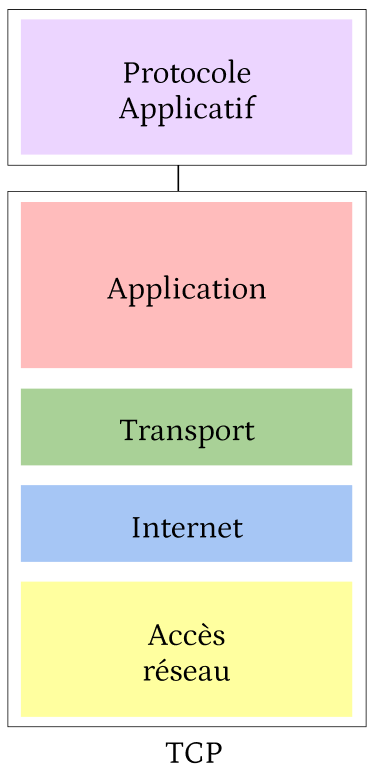
\includegraphics[width=5cm]{figures/protocole-appli.png}
    \par
    }

Avant de découvrir cela, 
Pour créer un protocole applicatif, il faut \emph{impérativement} passer par l'utilisation de socket permettant la création d'un canal de communication. \textbf Il faut toute fois définir quel mode souhaite on utilisé :
\begin{itemize}
     \item \textbf{Mode connecté}
     \item \textbf{Mode non connecté (datagram)}
\end{itemize}

Ces deux modes sont bien différents l'un de l'autre, nous le verrons plus tard.

\section{Utilité d'un protocole applicatif}

Il y a différentes utilité d'implémenter un protocole applicatif sur un réseau, serveur tel que :
\begin{itemize}
     \item Le contrôle du trafic comme on le souhaite
     \item La vérification et détection des erreurs
     \item Flexibilité en fonction du cas d'utilisation
     \item Le serveur est sécurisé si bien configuré
\end{itemize}

Cela est principalement utile pour avoir un certain contrôle sur le flux qui est envoyé et détecter les problèmes qui peuvent arriver lors d'envoie sur le réseau.

